% Options for packages loaded elsewhere
\PassOptionsToPackage{unicode}{hyperref}
\PassOptionsToPackage{hyphens}{url}
%
\documentclass[
]{article}
\usepackage{lmodern}
\usepackage{amssymb,amsmath}
\usepackage{ifxetex,ifluatex}
\ifnum 0\ifxetex 1\fi\ifluatex 1\fi=0 % if pdftex
  \usepackage[T1]{fontenc}
  \usepackage[utf8]{inputenc}
  \usepackage{textcomp} % provide euro and other symbols
\else % if luatex or xetex
  \usepackage{unicode-math}
  \defaultfontfeatures{Scale=MatchLowercase}
  \defaultfontfeatures[\rmfamily]{Ligatures=TeX,Scale=1}
\fi
% Use upquote if available, for straight quotes in verbatim environments
\IfFileExists{upquote.sty}{\usepackage{upquote}}{}
\IfFileExists{microtype.sty}{% use microtype if available
  \usepackage[]{microtype}
  \UseMicrotypeSet[protrusion]{basicmath} % disable protrusion for tt fonts
}{}
\makeatletter
\@ifundefined{KOMAClassName}{% if non-KOMA class
  \IfFileExists{parskip.sty}{%
    \usepackage{parskip}
  }{% else
    \setlength{\parindent}{0pt}
    \setlength{\parskip}{6pt plus 2pt minus 1pt}}
}{% if KOMA class
  \KOMAoptions{parskip=half}}
\makeatother
\usepackage{xcolor}
\IfFileExists{xurl.sty}{\usepackage{xurl}}{} % add URL line breaks if available
\IfFileExists{bookmark.sty}{\usepackage{bookmark}}{\usepackage{hyperref}}
\hypersetup{
  pdftitle={Propagating Sequence Uncertainty into Downstream Analyses},
  pdfauthor={David Champredon, Devan Becker, Art Poon, Connor Chato},
  hidelinks,
  pdfcreator={LaTeX via pandoc}}
\urlstyle{same} % disable monospaced font for URLs
\usepackage[margin=1in]{geometry}
\usepackage{graphicx}
\makeatletter
\def\maxwidth{\ifdim\Gin@nat@width>\linewidth\linewidth\else\Gin@nat@width\fi}
\def\maxheight{\ifdim\Gin@nat@height>\textheight\textheight\else\Gin@nat@height\fi}
\makeatother
% Scale images if necessary, so that they will not overflow the page
% margins by default, and it is still possible to overwrite the defaults
% using explicit options in \includegraphics[width, height, ...]{}
\setkeys{Gin}{width=\maxwidth,height=\maxheight,keepaspectratio}
% Set default figure placement to htbp
\makeatletter
\def\fps@figure{htbp}
\makeatother
\setlength{\emergencystretch}{3em} % prevent overfull lines
\providecommand{\tightlist}{%
  \setlength{\itemsep}{0pt}\setlength{\parskip}{0pt}}
\setcounter{secnumdepth}{5}



% ==== GENERAL ====

\newcommand{\warning}[1]{\textbf{\textcolor{orange}{((#1))}}}
\newcommand{\comment}[1]{\textsl{\textcolor{cyan}{((#1))}}}
\newcommand{\eg}{\textit{e.g.,}\xspace}
\newcommand{\ie}{\textit{i.e.},\xspace}

% ==== SPECIFIC ====

\newcommand{\sq}[1]{\texttt{\textcolor{brown}{#1}}}

\newcommand{\sps}{\mathcal{B}} % sequence probability sequence
\newcommand{\nps}{\mathcal{S}} % nucleotide probability sequence
\newcommand{\nlps}{nucleotide-level probabilistic sequence\xspace}
\newcommand{\slps}{sequence-level probabilistic sequence\xspace}

\newcommand{\pr}[1]{\mathbb{P}(#1)}

\newcommand{\md}{\mathcal{M}} % Multinomial distribution
\newcommand{\pois}[1]{\mathrm{Poisson}\left(#1\right)}
\newcommand{\betadist}[1]{\mathrm{Beta}\left(#1\right)}


\usepackage{xspace}
\usepackage{xcolor}
\usepackage{float}
\usepackage[]{natbib}
\bibliographystyle{plainnat}

\title{Propagating Sequence Uncertainty into Downstream Analyses}
\author{David Champredon, Devan Becker, Art Poon, Connor Chato}
\date{}

\begin{document}
\maketitle
\begin{abstract}
Genetic sequencing is subject to many different types of errors, but
most analyses treat the resultant sequences as if they are perfect.
Since the process of sequencing is very difficult, modern machines rely
on significantly larger numbers of reads rather than making each read
significantly more accurate. Still, the coverage of such machines is
imperfect and leaves uncertainty in many of the base calls. Furthermore,
there are circumstances around the sequencing that can induce further
problems. In this work, we demonstrate that the uncertainty in
sequencing techniques will affect downstream analysis and propose a
straightforward (if computationally expensive) method to propagate the
uncertainty.\\
Our method uses a probabilistic matrix representation of individual
sequences which incorporates base quality scores and makes various
uncertainty propagation methods obvious and easy. With the matrix
representation, resampling possible base calls according to quality
scores provides a bootstrap- or prior distribution-like first step
towards genetic analysis. Analyses based on these re-sampled sequences
will include an honest evaluation of the error involved in such
analyses.\\
We demonstrate our resampling method on HIV and SARS-CoV-2 data. The
resampling procedures adds computational cost to the analyses, but the
large impact on the variance in downstream estimates makes it clear that
ignoring this uncertainty leads to invalid conclusions. For HIV data, we
show that phylogenetic reconstructions are much more sensitive to
sequence error uncertainty than previously believed, and for SARS-CoV-2
data we show that lineage designations via Pangolin are much less
certain than the bootstrap support would imply.
\end{abstract}

\hypertarget{intro}{%
\section{Intro}\label{intro}}

Extracting DNA/RNA from biological samples is a complex process that
involves many steps: extraction of the genetic material of interest
(avoiding contamination with foreign/unwanted genetic material); reverse
transcription (if RNA); DNA fragmentation of the genome into smaller
segments; amplification of the fragmented sequences using PCR;
sequencing the fragments (\eg with fluorescent techniques); putting back
the small fragments together by aligning them (de novo) or mapping them
to benchmark libraries. Errors can be introduced at each of these steps
for various reasons
\citep[\citet{oraweAccountingUncertaintyDNA2015}]{beerenwinkelUltradeepSequencingAnalysis2011}
and some errors can be quantified (\eg sequencing quality scores from
chromatographs).

When the phylogenic tree to infer is based on pathogen sequences
infecting hosts, the potential genetic diversity of the infection adds a
complexity in phylogeny reconstruction. Typical examples are
epidemiological studies reconstructing transmission trees from viral
genetic sequences (\eg HIV, HepC) sampled from infected patients.

The different sources of uncertainty described above impact our
observations of the actual genetic sequences. There are standard
approaches to deal with identifiable observation errors. Base calls that
are ambiguous (from equivocal chromatograph curves or because of genuine
polymorphisms) are assigned ambiguity codes (\eg Y for C or T, R for A
or G, etc.). Alignment methods are heuristic methods based on similarity
scores that generally do not quantify the uncertainty of alignment.
Methods to reconstruct phylogenies usually leave out the uncertainty
complexity and settle for sequences composed of the most frequent
nucleotides and/or ignore ambiguity codes (with some exceptions,
e.g.~\citet{depristoFrameworkVariationDiscovery2011}).

In 1998, \citet{ewingBaseCallingAutomatedSequencer1998} and
\citet{richterichEstimationErrorsRaw1998} both showed that estimates of
the base call quality (called Phred scores) can be an accurate estimate
of the number of errors that the machines at the time would make. Modern
machines still report these Phred scores, but methods for
adjusting/recalibrating these scores for greater accuracy have been
proposed \citep[\citet{depristoFrameworkVariationDiscovery2011},
\citet{liSNPDetectionMassively2009}]{liAdjustQualityScores2004} For most
analyses, these scores are used to censor the base calls (i.e., label
them ``N'' rather than A, T, C, or G) if the base call error probability
is too high or there are too few reads and a given location. It is
commonplace to remove the sequence from analysis if the total sequence
error probability is too high \citep[see,
e.g.,][\citet{robaskyRoleReplicatesError2014},
\citet{oraweAccountingUncertaintyDNA2015}]{doroninaPhylogeneticPositionEmended2005}.
The error probability is deemed too high based on a strict threshold
(e.g.~1\% chance of error), but these thresholds aren't necessarily
standard across studies.

Some studies have incorporated the error probabilities using genome
likelihoods. \citet{depristoFrameworkVariationDiscovery2011} and
\citet{gompertHierarchicalBayesianModel2011} incoporate the adjusted
Phred scores into a likelihood framework that allows them to more
accurately estimate population-level allele distributions.
\citet{fumagalliQuantifyingPopulationGenetic2013a} present a new
estimator for population genetic diversity based on such analyses.
\citet{kuoEAGLEExplicitAlternative2018} use genome likelihoods to
perform hypothesis tests that evaluate whether a given genome sequence
is consistent with a given alternative sequence, after accounting for
the errors. As with any parametric model-based approach, genome
likelihoods use assumptions about the errors in order to make
conclusions about the underlying patterns.

Few other authors have considered the uncertainty present in the
sequences in downstream analyses. One notable exception is
\citet{oraweAccountingUncertaintyDNA2015}, who suggest methods for
propagating sequence-level uncertainty into determining whether two
subjects have the same alleles as well as incorporating the
sequence-level uncertainty into confidence intervals for allele
frequency.

In our work, we present a simple, general framework that can be
incorporated into any analysis of genetic sequence data. This framework
involves converting the uncertainty scores into a matrix of
probabilities, and repeatedly sampling from this matrix and using the
resultant samples in downstream analysis. Unlike likelihood-based
approaches, we do not make assumptions about the underlying patterns in
the data. In doing so, we gain generalizability at the expense of
computation time. Our technique is amenable to any appropriate quality
score adjustments prior to building the uncertainty matrix.

\hypertarget{methods}{%
\section{Methods}\label{methods}}

\hypertarget{probabilistic-representation-of-sequences}{%
\subsection{Probabilistic Representation of
Sequences}\label{probabilistic-representation-of-sequences}}

Here, we describe two theoretical frameworks to model sequence
uncertainty at the \emph{nucleotide level} or at the
\emph{sequence level}. In both frameworks, the sequence of nucleotides
from a biological sample is not treated as a certain observation, but as
a collection of possible sequences.

\hypertarget{nucleotide-level-uncertainty}{%
\subsubsection{Nucleotide-level
uncertainty}\label{nucleotide-level-uncertainty}}

To represent the uncertainty at each location along the genome, we
introduce following matrix:

\begin{equation}
\nps = \bordermatrix{   & 1 & 2 & \ldots & \ell \cr
                \sq{A} & \nps_{A, 1} & \nps_{A, 2} & \ldots & \nps_{A, \ell} \cr
                \sq{C} & \nps_{C, 1} & \nps_{C, 2} & \ldots & \nps_{C, \ell} \cr
                \sq{G} & \nps_{G, 1} & \nps_{G, 2} & \ldots & \nps_{G, \ell} \cr
                \sq{T} & \nps_{T, 1} & \nps_{T, 2} & \ldots & \nps_{T, \ell} \cr 
                \sq{-} & \nps_{x, 1} & \nps_{x, 2} & \ldots & \nps_{x, \ell} \cr 
}\label{eq:nps}
\end{equation}

Each column represents the nucleotide position, each row one of the four
nucleotide \sq{A,C,G,T} as well as an empty position ``\sq{-}''" that
symbolizes a genuine deletion (not caused by missing data). Hence,
\(\nps\) is a \(5\times\ell\) matrix. Its elements represent the
probability that a nucleotide is at given position:

\begin{equation}
\nps_{\sq{n},j} = \pr{\text{nucleotide \sq{n} is at position }j}
\end{equation} with the special case for a deletion:

\begin{equation}
\nps_{\sq{-},j} = \pr{\text{empty position }j}
\end{equation} Note that we have for all \(1\leq j \leq \ell\):
\begin{equation}
\sum_{n\in \{ \sq{A,C,G,T,-} \} } \nps_{n, j} = 1
\end{equation} Also, the sequence length is stochastic if
\(\nps_{\sq{-},i}>0\) for at least one \(i\). The probability that the
sequence has the maximum length \(\ell\) is
\(\prod_{i=1}^\ell (1-\nps_{\sq{-},i})\). We call the matrix \(\nps\)
the \emph{\nlps} of a biological sample. The nucleotide (or deletion)
drawn at each position is independent from all the others, so there are
\(5^\ell\) possible different sequences for a given probabilistic
nucleotide sequence, but these sequences are \emph{not} equally
probable.

\hypertarget{sequence-level-uncertainty}{%
\subsubsection{Sequence-level
uncertainty}\label{sequence-level-uncertainty}}

Out of the \(5^\ell\) possible sequences, the nucleotide uncertainty may
assign a positive probability to sequences that are not biologically
possible. As an alternative representation and to reduce the space of
possible sequences, let's assume we have enough information (either
directly observed from data or simulated) to generate a set of sequences
\(\sps = (\sps_i)_{i\in\{1\ldots m\} }\) of all \(m\) biologically
possible sequences. Note that the \(\sps_i\) do not have necessarily the
same length. The observed genetic sequence, \(s\), is a sample from a
specified distribution \(a\): \begin{equation}
\pr{s = \sps_i} = a(i)
\end{equation} We call the set \(\sps\) the \emph{\slps}. Note that,
because \(a\) is a distribution, we must have \(\sum_{i=1}^m a(i) = 1\).

If we have the following \nlps: \[
\nps = 
\bordermatrix{
& \scriptscriptstyle{1} & \scriptscriptstyle{2}& \scriptscriptstyle{3}& \scriptscriptstyle{4} & \scriptscriptstyle{5} & \scriptscriptstyle{6} \cr
\sq{A} & 0.9 & 0.05   & 0.99 & 0 & 0 & 0.6\cr
\sq{C} & 0   & 0.8 & 0 & 0 & 0.1 & 0.1\cr
\sq{G} & 0.1 & 0.15 & 0 & 0.3 & 0.9 & 0\cr
\sq{T} & 0 & 0 & 0.01 & 0.7 & 0 & 0.3\cr
\sq{-} & 0 & 0 & 0 & 0 & 0 & 0\cr
}
\] then there are \(2\times 3 \times 2^3 \times 3 = 144\) possible
sequences. The most likely is the one having the highest nucleotides
probabilities: \sq{ACATGA} with probability 0.2694
(\(0.9\times 0.8\times 0.99 \times 0.7 \times 0.9 \times 0.6\)).

If there is a positive probability of deletion for at least one
position, then the sequence has a variable length. Let's take the same
example as above, but adding one possible empty position:

\[
\nps = 
\bordermatrix{
&\scriptscriptstyle{1} & \scriptscriptstyle{2}& \scriptscriptstyle{3}& \scriptscriptstyle{4} & \scriptscriptstyle{5} & \scriptscriptstyle{6} \cr
\sq{A} & 0.9 & 0.05   & 0.99 & 0 & 0 & 0.6\cr
\sq{C} & 0   & 0.8 & 0 & 0 & 0.1 & 0.1\cr
\sq{G} & 0.1 & 0.15 & 0 & 0.2 & 0.9 & 0\cr
\sq{T} & 0 & 0 & 0.01 & 0.7 & 0 & 0.3\cr
\sq{-} & 0 & 0 & 0 & 0.1 & 0 & 0\cr
}
\]

\noindent Like above, there is still a 0.2694 probability that the
sequence is \sq{ACATGA}, but now there is a chance that position 4 is
deleted. For example, with probability 0.038 the sequence is
\sq{ACA-GA}.

Below is an example for a \slps \(\sps\):

\begin{table}[H]
\begin{center}
\begin{tabular}{lc}
\hline
\textbf{sequence} & $a$ \\
\hline
\sq{ACATGA} & 0.60 \\
\sq{ACATCA} & 0.12 \\
\sq{AGATCA} & 0.15 \\
\sq{ACAGA}  & 0.05 \\
\sq{GCATGA} & 0.08 \\
\hline
\end{tabular}
\end{center}
\label{default}
\end{table}

\% Sampling from \(\sps\), we will have for example \sq{ACATCA} \(12\%\)
of the time. Large genomes, such as SARS-CoV-2, will result in vanishly
small probabilities for all sequences, and thus work on the log scale is
often preferred.

\hypertarget{deletions-and-insertions}{%
\subsection{Deletions and Insertions}\label{deletions-and-insertions}}

By construction, the \nlps must be defined with its longest possible
length. Deletions are naturally modelled with our representation but
insertions have to be modelled using deletion probability.

Consider the following \nlps: \begin{equation}
\label{eq:indel}
\nps = 
\bordermatrix{
&\scriptscriptstyle{1} & \scriptscriptstyle{2}& \scriptscriptstyle{3}& \scriptscriptstyle{4} & \scriptscriptstyle{5} & \scriptscriptstyle{6} \cr
\sq{A} & 0 & 0   & 1 & 0    & 1 & 0\cr
\sq{C} & 1 & 0    & 0 & 0    & 0 & 0\cr
\sq{G} & 0 & 0.99 & 0 & 0    & 0 & 0\cr
\sq{T} & 0 & 0    & 0 & 0.01 & 0 & 1\cr
\sq{-} & 0 & 0.01 & 0 & 0.99 & 0 & 0\cr
}
\end{equation}

The low deletion probability for position 2 is straightforward to
interpret: about 1\% of the time, nucleotide \sq{G} at position 2 is
deleted. The high deletion probability for position 4 means there is a
1\% chance of a \sq{T} insertion at this position.
\autoref{tab:indelexample} illustrates this.

\begin{table}[H]
\caption{Representation of insertions and deletions from $\nps$ defined in \eqref{eq:indel}}
\begin{center}
\label{tab:indelexample}
\begin{tabular}{ll}
\hline
\textbf{sequence} & \textbf{frequency} \\
\hline
\sq{CGAAT}  & common, 98\% of the time \\
\sq{CAAT}   & rare (1\% frequency) \sq{G} deletion at position 2,  \\
\sq{CGATAT} & rare (1\% frequency) \sq{T} insertion at position 4 \\
\sq{CATAT} & very rare (0.01\% frequency) deletion and insertion  \\
\hline
\end{tabular}
\end{center}
\end{table}

The representation of deletions and insertions with a \slps (not
nucleotide-level) is straightforward because in this framework the
sequences are explicitly written out, so are their deletions/insertions.

\hypertarget{constructing-the-uncertainty-matrix}{%
\subsection{Constructing The Uncertainty
Matrix}\label{constructing-the-uncertainty-matrix}}

Fragment sequencing error is an error that is quantified with quality
(or ``Phred'') score attributed to each base call from sequencing
instrument. The quality score \(Q\) is directly related to the error
probability: \(\epsilon = 10^{-Q/10}\).
\cite{ewingBaseCallingAutomatedSequencer1998} (where \(Q\) typically
ranges between 1 and 60). The FASTQ file format is the standard
representation for combining sequence and observation error. Hence, the
uncertainty associated to the base call is quantified by defining the
probability that the observed nucleotide is the correct one:
\begin{equation}
\label{eq:basecall}
\pr{\text{nucleotide}=X \,\,|\,\, \text{observed nucleotide} = X} = 1 - \epsilon
\end{equation}

Unfortunately, this base-call probability relates to only one
\emph{focal} nucleotide and we have no information on the probability
for the three other possible nucleotides. Hence, we must make a
modelling choice regarding the distribution of the remaining
probabilities.

\hypertarget{sam-files}{%
\subsubsection{SAM Files}\label{sam-files}}

Massive parallel sequencing platforms (\eg Illumina, Oxford Nanopores,
etc.) provide a large number of short reads sequences of the biological
sample of interest. The length of those short reads are typically much
smaller than the genome sequenced, so they have to be aligned and stitch
together in order to re-assemble the full genome sequence. The short
reads are typically stored in FASTQ files where the observation error of
each nucleotide (estimated by the sequencing platform itself)) is
indicated by its Phred score. The alignment and assembly of the short
reads is performed by software (internal to the sequencing platform or
not \comment{check this. Examples?}) and generates a SAM file
\comment{ref} that efficiently stores the alignment information. The
assembly of the short reads in the SAM file can be represented in as an
array where the columns are the nucleotide positions. The short reads
are ``stacked'' vertically according to the alignment. The number of
short reads stacked for a given nucleotide gives the ``coverage'' of
that position. See \autoref{fig:sam} for an illustration of this SAM
file representation.

\begin{figure}[ht]
\centering
    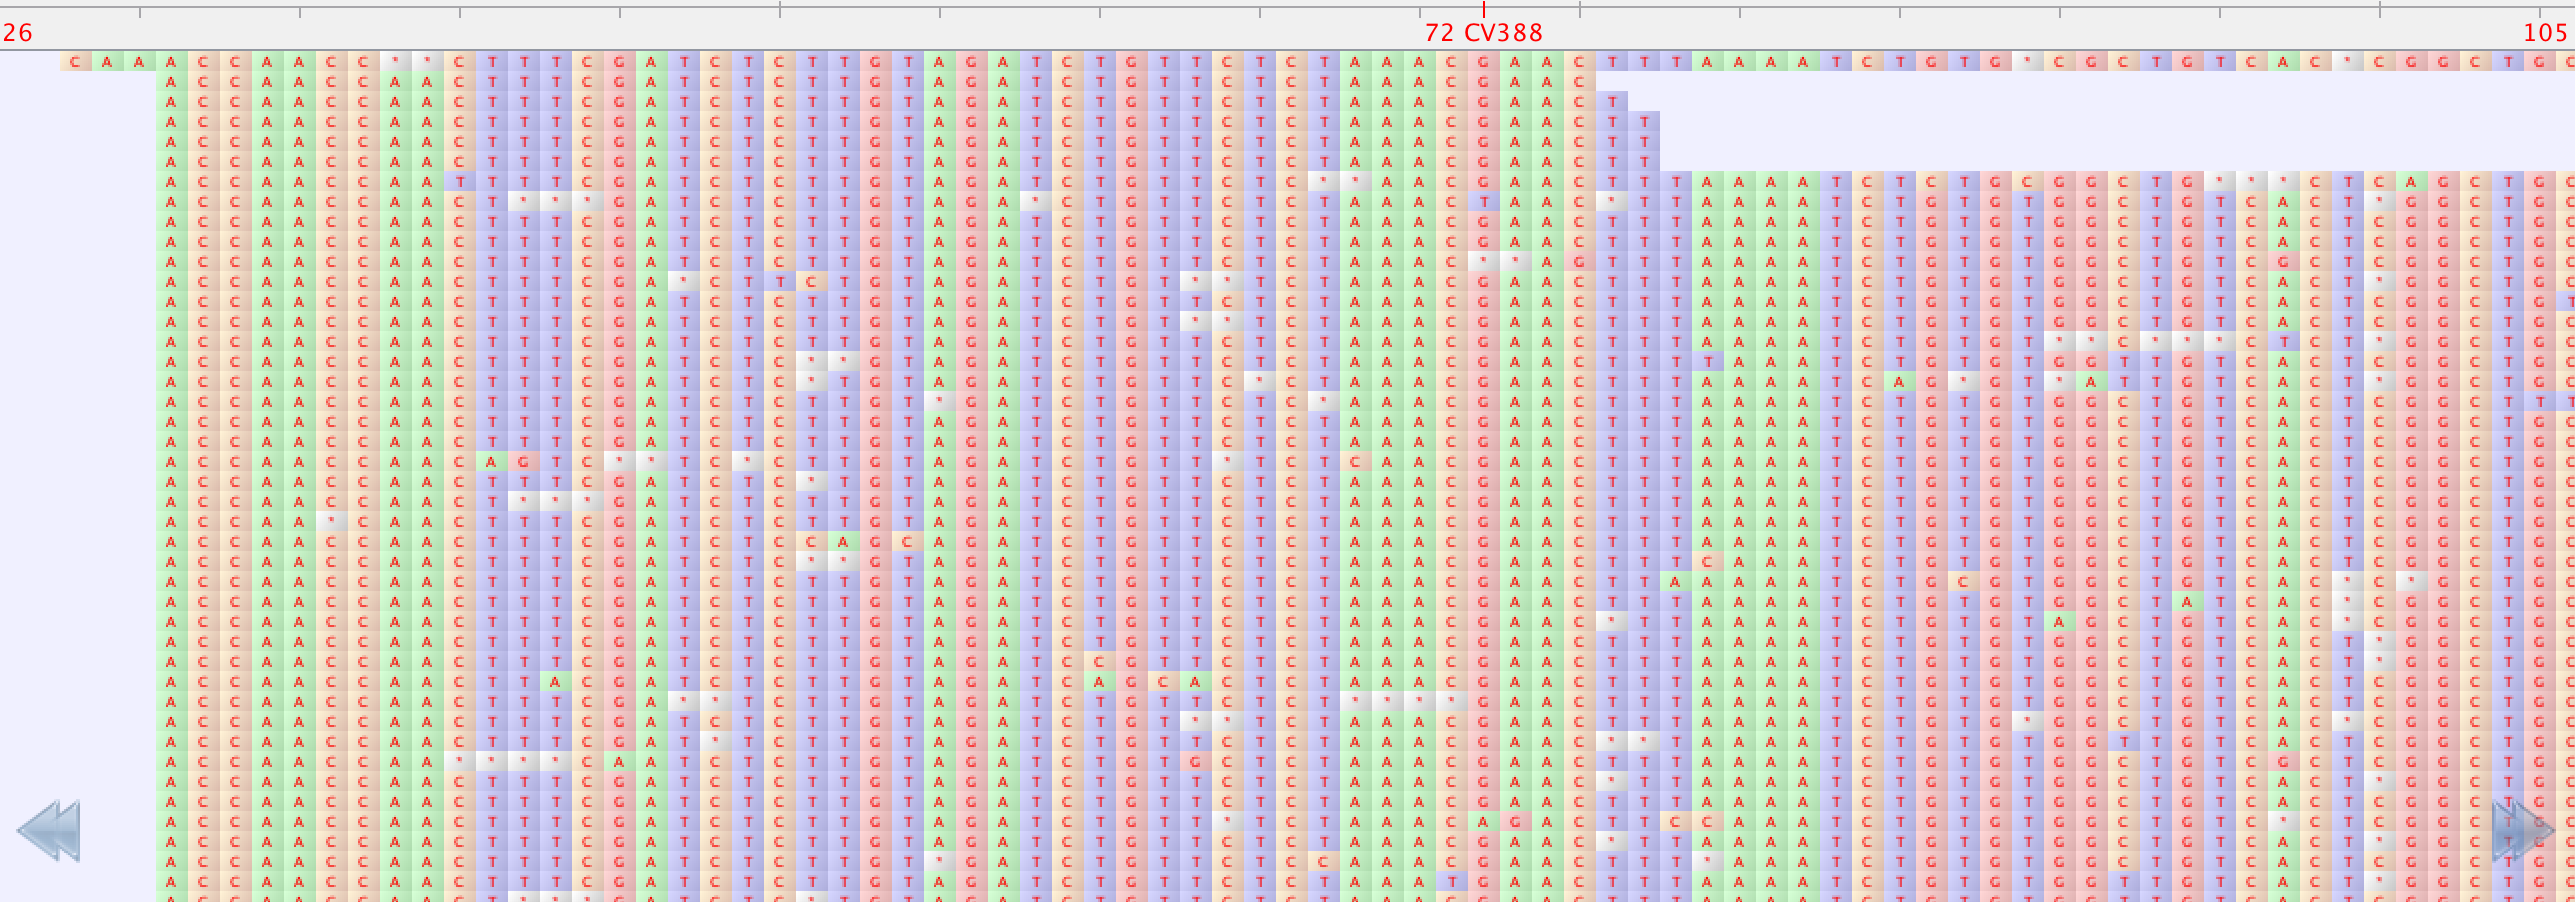
\includegraphics[width=0.99\textwidth]{../ms/figs/sam-tablet.png}
\caption{\textbf{SAM file graphical representation.} The software Tablet \comment{ref } was used. Each base call is colour coded so that base calls that disagree with the consesnsu are obvious. The 72th nucleotide in this alignment has a coverage of 388 reads.}
\label{fig:sam}
\end{figure}

The nucleotide-level probabilistic sequence can be constructed from this
alignment. The algorithm that we suggest is as follows.

We begin by initializing an empty \(5\times\ell\) matrix \(\nps`\). Each
label in Figure \ref{fig:sam} has an associated probability score. These
labels denote a row in \(\nps\), and their location on the genome
denotes the columns, say (\(\sq{A}, j\)). At this entry, we add the
corresponding quality score to whatever was there before.

By this construction, the sum of each column represents the coverage at
that location. Dividing each entry of \(\nps'\) by the sum of that
column results in \(\nps\). For our proposed propagation methods, it is
convenient to work with \(\nps`\) until probabilities are necessary.

\hypertarget{fastq-files}{%
\subsubsection{FASTQ files}\label{fastq-files}}

For most published genome sequences, the short read files are not
available. It is common to find the so-called consensus sequence, which
is the sequence that represents the most commonly called base at each
location, along with a single quality score for each location. The
methods for obtaining Phred scores when converting a SAM file to a
consensus FASTQ differ by software
\citep[\citet{keithSimulatedAnnealingAlgorithm2002},
\citet{liMappingShortDNA2008}]{liAdjustQualityScores2004}, but generally
involve a computation that includes all of the Phred scores of the bases
that agree with the consensus (\eg if the short reads have \sq{A} with
Phred of 30, \sq{A} with a Phred of 31, and \sq{C} with phred of 15,
then the Phred scores of 30 and 31 are combined).

\hypertarget{propogation-of-uncertainty-via-resampling}{%
\subsection{Propogation of Uncertainty via
Resampling}\label{propogation-of-uncertainty-via-resampling}}

\hypertarget{sequence-level-uncertainty-seqleveluncertaint}{%
\subsection{Sequence-level Uncertainty
(seqLevelUncertaint)}\label{sequence-level-uncertainty-seqleveluncertaint}}

\hypertarget{reducing-computational-burden-via-sequence-level-uncertainty}{%
\subsubsection{Reducing Computational Burden via Sequence-level
Uncertainty}\label{reducing-computational-burden-via-sequence-level-uncertainty}}

\hypertarget{application-to-sars-cov-2}{%
\section{Application to SARS-CoV-2}\label{application-to-sars-cov-2}}

\hypertarget{data}{%
\subsection{Data}\label{data}}

The data for this application were downloaded from NCBI's SRA web
interface. Results were filtered to only include runs that had bam
files. To select which runs to download, a selection of 5-10 files from
each of 20 non-sequential search result pages was chosen. Once
collecting the run accession numbers from the search results, an R
script was run to download the relevant files and check that all
information was complete. 23 out of 300 files were labelled incomplete
due to having too few reads (possibly because the download timed out) or
not containing a CIGAR string.

There was no particular reason for choosing any given file, but the
resulting data should not be viewed as a random sample. Each result page
likely includes several runs from the same study, and runs were chosen
arbitrarily within each result page. We were not attempting a completely
random sampling strategy, we simply wanted a collection of runs on which
to demonstrate our methods.

\hypertarget{pangolearn}{%
\subsection{PANGOlearn}\label{pangolearn}}

\hypertarget{possibly-constructing-trees}{%
\subsection{(Possibly) constructing
trees}\label{possibly-constructing-trees}}

\hypertarget{variant-hypothesis-testing-via-mc}{%
\subsection{Variant hypothesis testing via
MC}\label{variant-hypothesis-testing-via-mc}}

\hypertarget{conclusions}{%
\section{Conclusions}\label{conclusions}}

\hypertarget{for-pangolin}{%
\subsection{For Pangolin}\label{for-pangolin}}

\hypertarget{for-phylogenetics-in-general}{%
\subsection{For phylogenetics in
general}\label{for-phylogenetics-in-general}}

\hypertarget{for-analysis-of-genetic-data}{%
\subsection{For analysis of genetic
data}\label{for-analysis-of-genetic-data}}

\begin{itemize}
\tightlist
\item
  Our method does not preclude tertiary analyses to test for systematic
  errors or deviations from a Mendelian inheritance pattern assumption.
\end{itemize}

  \bibliography{supbib.bib}

\end{document}
